\documentclass{beamer}
%\usepackage{beamerthemeMarburg}
%\usepackage{beamerthemeboxes}
%\usepackage{beamerthemePittsburgh}
\usepackage{amsmath, amssymb,multicol}
\usepackage{concrete}
\usepackage{graphicx}
\usepackage{epstopdf}
\usepackage{url}
\usepackage[all,arc]{xy}
\usepackage{enumerate}
\usepackage{mathrsfs}
\usepackage{relsize}
\newcommand{\R}{\mathbb{R}}
\newcommand{\tr}{\text{Tr}}
\newcommand{\ra}[1]{\renewcommand{\arraystretch}{#1}}

\setbeamertemplate{frametitle} {\begin{centering}\smallskip \insertframetitle\par \smallskip\end{centering}}
\setbeamertemplate{itemize item}{$\bullet$}
\setbeamertemplate{navigation symbols}{}
%\setbeamertemplate{footline}[text line]{%
%	\hfill\strut{%
%	\scriptsize\sf\color{black!60}%
%	\quad\insertframenumber
%	}%
%	\hfill}

\definecolor{DarkFern}{HTML}{407428}
\definecolor{DarkCharcoal}{HTML}{4D4944}
\colorlet{Fern}{DarkFern!85!white}
\colorlet{Charcoal}{DarkCharcoal!90!white}
\colorlet{LightCharcoal}{Charcoal!50!white}
\colorlet{AlertColor}{orange!80!black}
\colorlet{DarkRed}{red!70!black}
\colorlet{DarkBlue}{blue!70!black}
\colorlet{DarkGreen}{green!70!black}
\definecolor{MyColor}{HTML}{101BD2}
\colorlet{lightMyColor}{MyColor!70!white}


% Use the colors:

%\setbeamercolor{title}{fg=Fern}
\setbeamercolor{title}{fg=MyColor}
%\setbeamercolor{frametitle}{fg=Fern}
\setbeamercolor{frametitle}{fg=lightMyColor}
\setbeamercolor{normal text}{fg=Charcoal}
\setbeamercolor{block title}{fg=black,bg=MyColor!70!white}
\setbeamercolor{block body}{fg=black,bg=MyColor!35!white}
\setbeamercolor{alerted text}{fg=AlertColor}
\setbeamercolor{itemize item}{fg=lightMyColor}
\setbeamercolor{enumerate item}{fg=lightMyColor}


\title{Not `Won't you be my neighbor?' \\ But `Should you be my neighbor?'}
\subtitle{\textcolor{lightMyColor}{Optimal Information Gathering in Social Networks}}
\author{Eleanor Brush}

\begin{document}

\frame{\titlepage}

\begin{frame}

\begin{center}
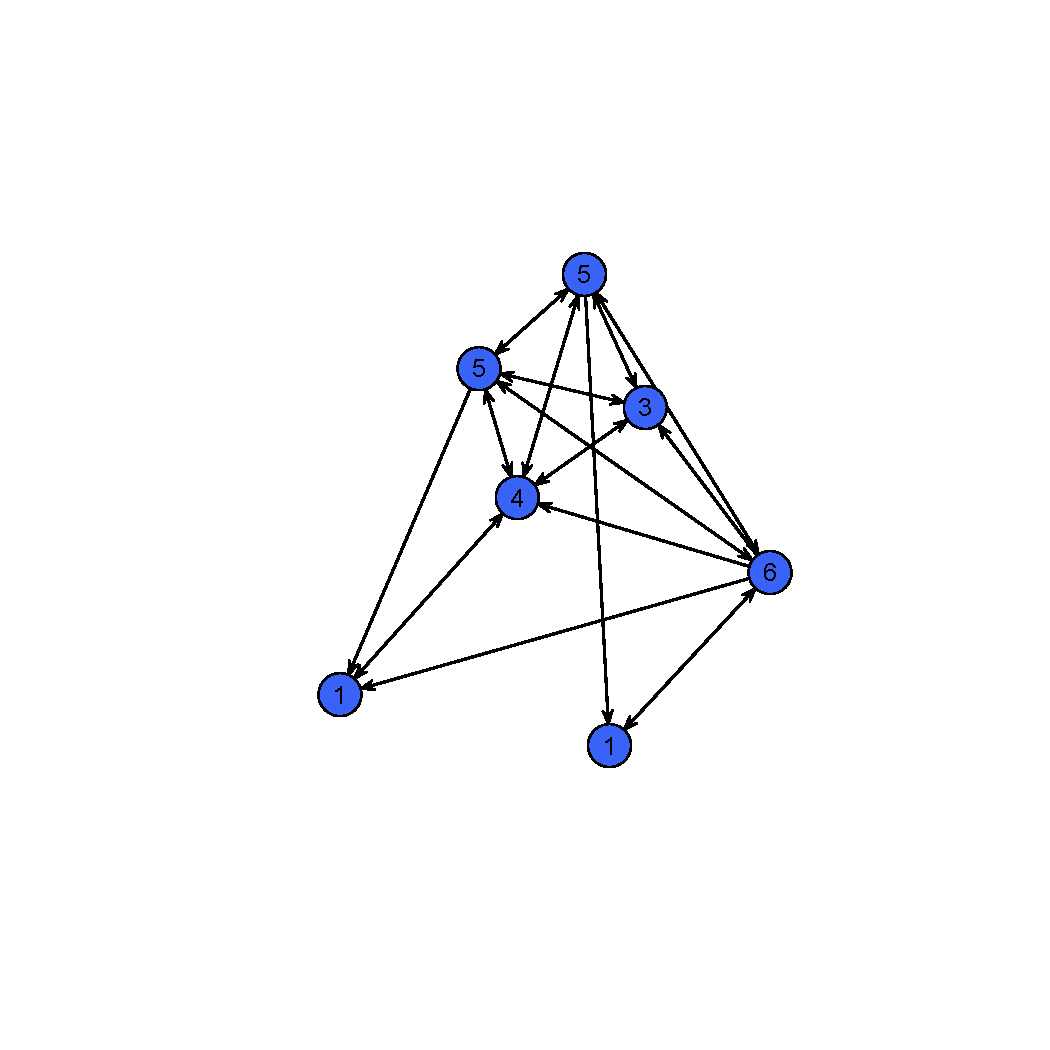
\includegraphics[width=.8\textwidth]{social_network.pdf}
\end{center}

\end{frame}

\begin{frame}

\begin{center} {\Large What's the optimal way to gather information from a social network?}\end{center}

\begin{enumerate}
\pause \item a criterion of performance
\pause \item a strategy to maximize that criterion
\end{enumerate}
\end{frame}

\begin{frame}
\frametitle{Overview}
\begin{enumerate}
\item a criterion for the whole network
\item a criterion for individuals
\item consequences of and strategy for optimizing individual performance
\item a measure of informational burden
\item future directions
\end{enumerate}
\end{frame}


\begin{frame}

\[ \scalebox{1.8}{$\dot{x}_i(t)=\sum_jw_{ij}\big(x_j(t)-x_i(t)\big)+\xi_i(t)$}\]
\\\[ \scalebox{1.25}{ where $\sum_jw_{ij} =1$ and $\xi_i(t)\sim N(0,1)$ i.i.d.} \]
\vspace{25pt}\[ \scalebox{1.5}{ $\Longrightarrow$ consensus with every $x_i=c$} \]

\end{frame}

\begin{frame}

\[ \scalebox{1.8}{$ \dot{x}(t)=-Lx(t)+\xi(t)$ }\]
\[\scalebox{1.25}{ where $L_{ij}=\left\{ \begin{array}{cccc} 1 & \text{ if } i=j \\ -w_{ij} & \text{ if } i\neq j \end{array}\right.$ }\]
%Without noise, an equilibrium is reached when $Lx=0$.  
\vspace{25pt}\[ \scalebox{1.5}{ $\Longrightarrow$ consensus with $x\propto \vec{1}$} \]
\end{frame}

\begin{frame}
\begin{center}
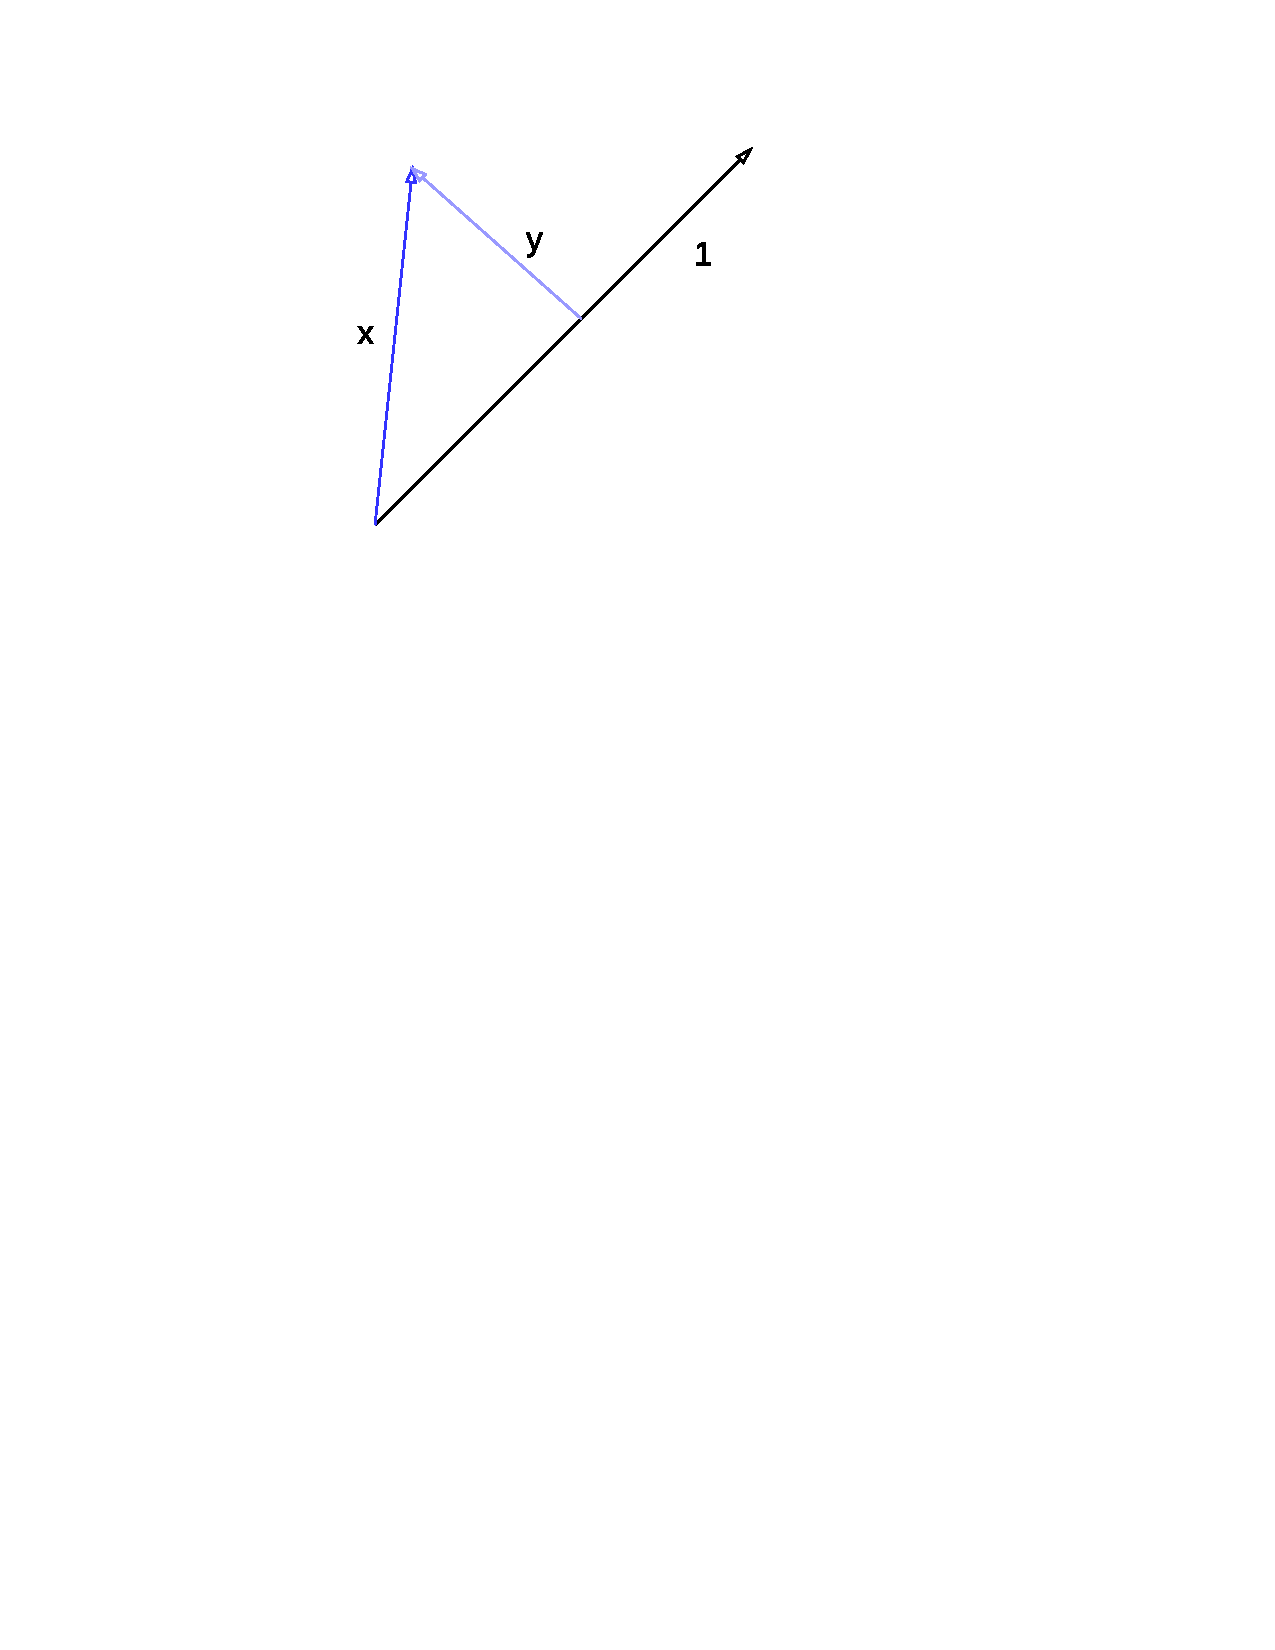
\includegraphics[scale=.8]{vectors.pdf}
\end{center}
\end{frame}

\begin{frame}
\frametitle{Deviation from Consensus}
Define the orthogonal transformation $Q\in\R^{n-1\times n}$ with 
\begin{enumerate}
\item $Q\vec{1}=0$
\item $QQ^T=I_{n-1}$ and 
\item $Q^TQ=I_n-\frac{1}{n}\vec{1}\times \vec{1}^T$
\end{enumerate}
Define $\textcolor{MyColor}{y=Qx}$ and $\textcolor{MyColor}{\overline{L}=QLQ^T}$.

$$\Longrightarrow \dot{y}(t)=-\overline{L}y(t)+Q\xi(t)$$

\vspace{50pt}\tiny{Starling flock networks manage uncertainty in consensus at low cost, \\George F. Young, Luca Scardovi, Andrea Cavagna, Irene Giardina, and Naomi E. Leonard. 2012.}

\end{frame}

\begin{frame}
\frametitle{Network Optimization}
One measure of performance:
$$H(L)=\lim_{t\to\infty}E[||y(t)||]$$

Objective: choose the number of neighbors $m$ that maximizes $$\frac{1}{\left(\frac{H}{\sqrt{N}}\right)m}$$

\end{frame}

\begin{frame}
\begin{center}
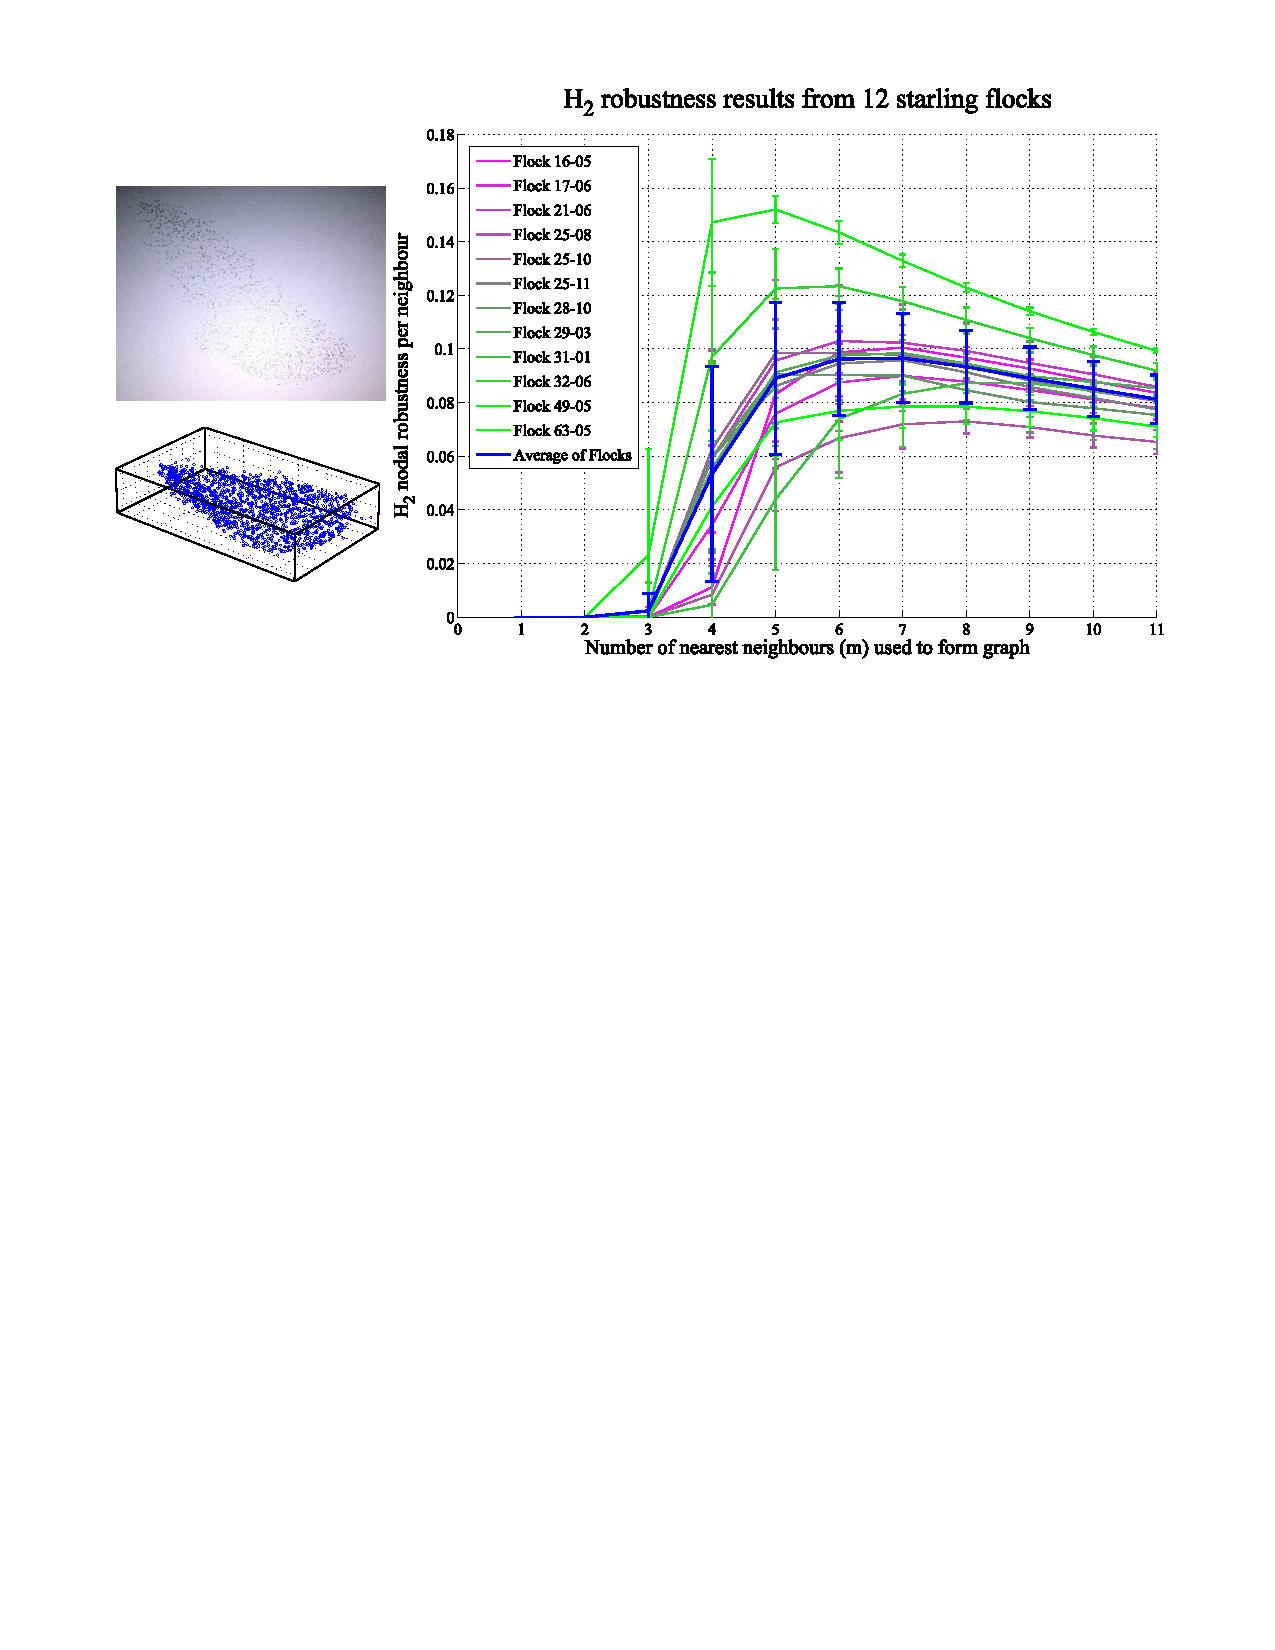
\includegraphics[width=\textwidth]{starling_robustness.pdf}
\end{center}
\vspace{30pt}\tiny{Starling flock networks manage uncertainty in consensus at low cost, \\ \vspace{-6pt} George F. Young, Luca Scardovi, Andrea Cavagna, Irene Giardina, and Naomi E. Leonard. 2012.}
\end{frame}

\begin{frame}
\frametitle{Learning about the world}
One node gets an external signal so that 
\begin{align*}
x_i(t)&=\text{signal } \text{ for all } t \text{ and }
\\ \dot{x}_j(t)&=\sum_kw_{jk}\big(x_k(t)-x_j(t)\big)+\xi_j(t) \text{ for } k\neq i
\\ \delta_j(t)&:=\text{ signal } -x_j(t)
\\ \Rightarrow \dot{\delta}(t)&=-L^i\delta(t)+L^i\xi(t) 
\\ \text{ where } L^i&=L \text{ without the $i^{th}$ row and column}
\end{align*}
\end{frame}

\begin{frame}

We can approximate $\delta_j(t)$ with $$\delta_j(t)\sim e^{-\lambda^it}v_j^i$$ where $\lambda^i$ is the smallest eigenvalue of $L^i$ and $v^i$ is its eigenvector.

\end{frame}

\begin{frame}
\begin{block}{{\small Deviations}}{
{\small from consensus: $\dot{y}(t)=-\overline{L}y(t)+Q\xi(t) $}
\\{\small from external signal: $\dot{\delta}(t)=-L^i\delta(t)-L^i\xi(t)$}
}\end{block}
Minimizing 
$$\delta_j(t)\sim e^{-\lambda^it}v_j^i$$
\textcolor{lightMyColor}{\emph{usually}} optimizes consensus in the whole group because 
\begin{enumerate}
\item the rate of convergence to consensus is given by $\overline{\lambda}$, the smallest eigenvalue of $\overline{L}$, and $\lambda^i\leq\overline{\lambda}$
\invisible<1>{\item $\lim_{t\to\infty}E[||\delta(t)||]\geq \lim_{t\to\infty}E[||y(t)||]$}
\end{enumerate}
\end{frame}

\begin{frame}
\begin{center}
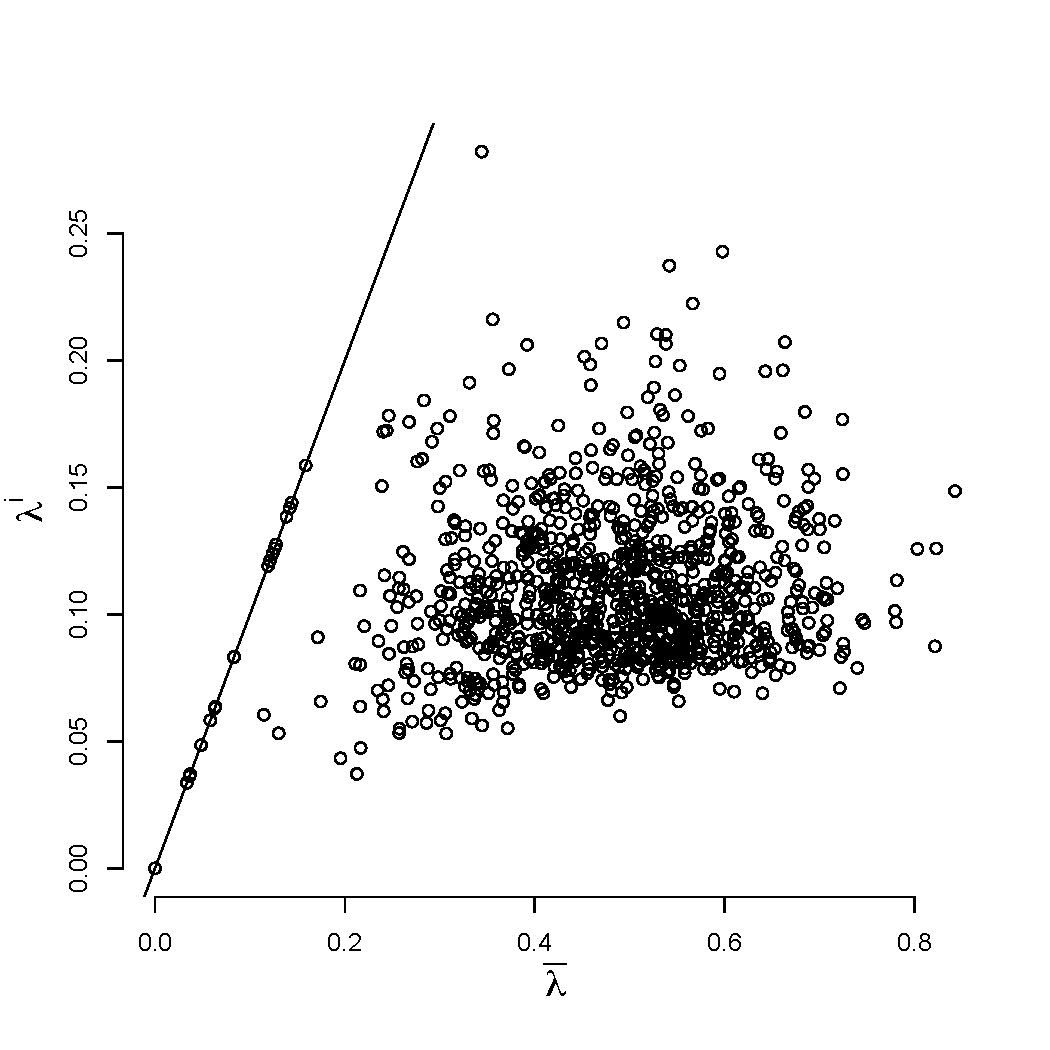
\includegraphics[width=.8\textwidth]{eigenvalue_comparison}
\end{center}
\end{frame}


\begin{frame}
\begin{block}{{\small Deviations}}{
{\small from consensus: $\dot{y}(t)=-\overline{L}y(t)+Q\xi(t) $}
\\{\small from external signal: $\dot{\delta}(t)=-L^i\delta(t)-L^i\xi(t)$}
}\end{block}
Minimizing 
$$\delta_j(t)\sim e^{-\lambda^it}v_j^i$$
\textcolor{lightMyColor}{\emph{usually}} optimizes consensus in the whole group because 
\begin{enumerate}
\item the rate of convergence to consensus is given by $\overline{\lambda}$, the smallest eigenvalue of $\overline{L}$, and $\lambda^i\leq\overline{\lambda}$
\item $\lim_{t\to\infty}E[||\delta(t)||]\geq \lim_{t\to\infty}E[||y(t)||]$
\end{enumerate}
\end{frame}

\begin{frame}
\begin{center}
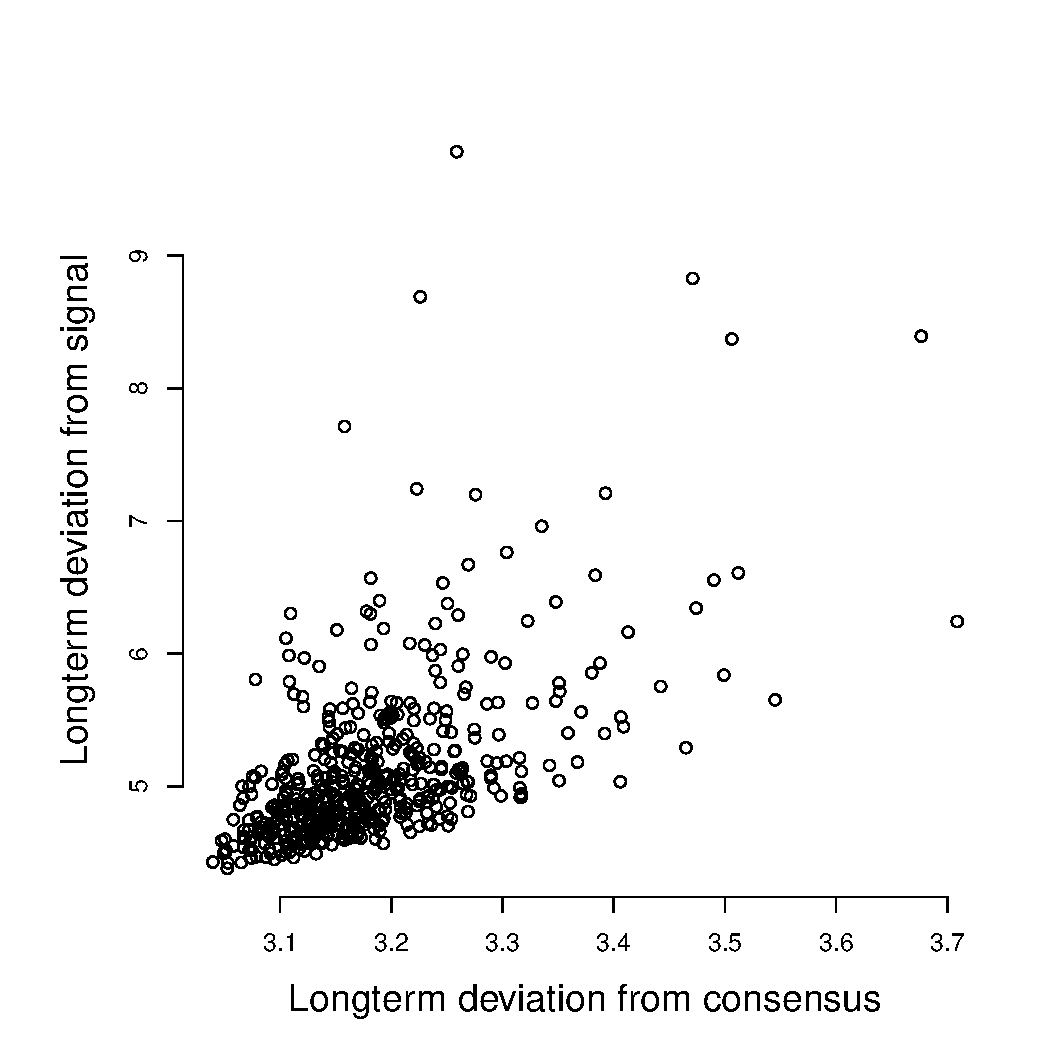
\includegraphics[width=.8\textwidth]{deviations.pdf}
\end{center}
\end{frame}

\begin{frame}
\frametitle{Individual Optimization}
Objective: each node $j$ wants to minimize $s_j=\langle e^{-\lambda^i}v_j^i \rangle _i$
\end{frame}


\begin{frame}
\begin{center}
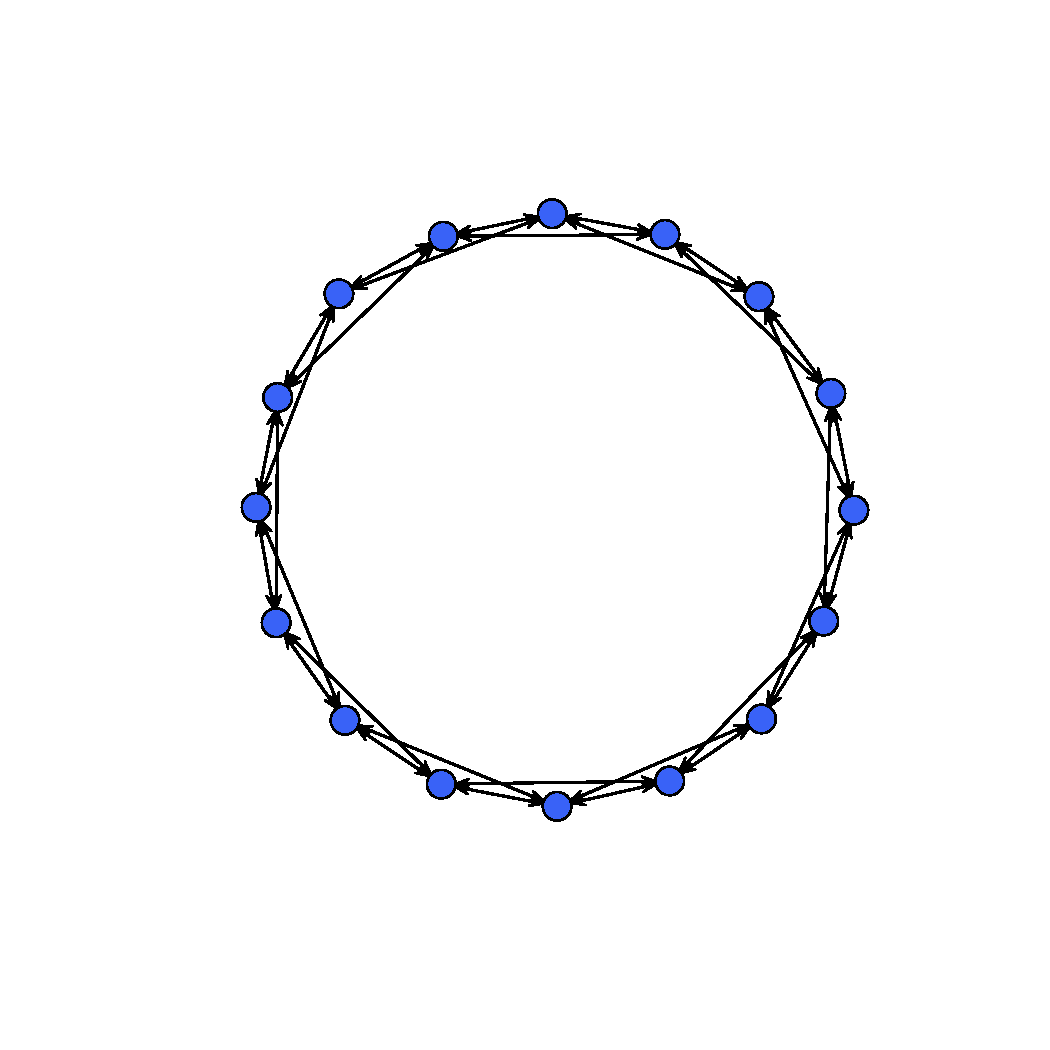
\includegraphics[width=.6\textwidth]{circle.pdf}
\end{center}
\end{frame}

\begin{frame}
\begin{center}
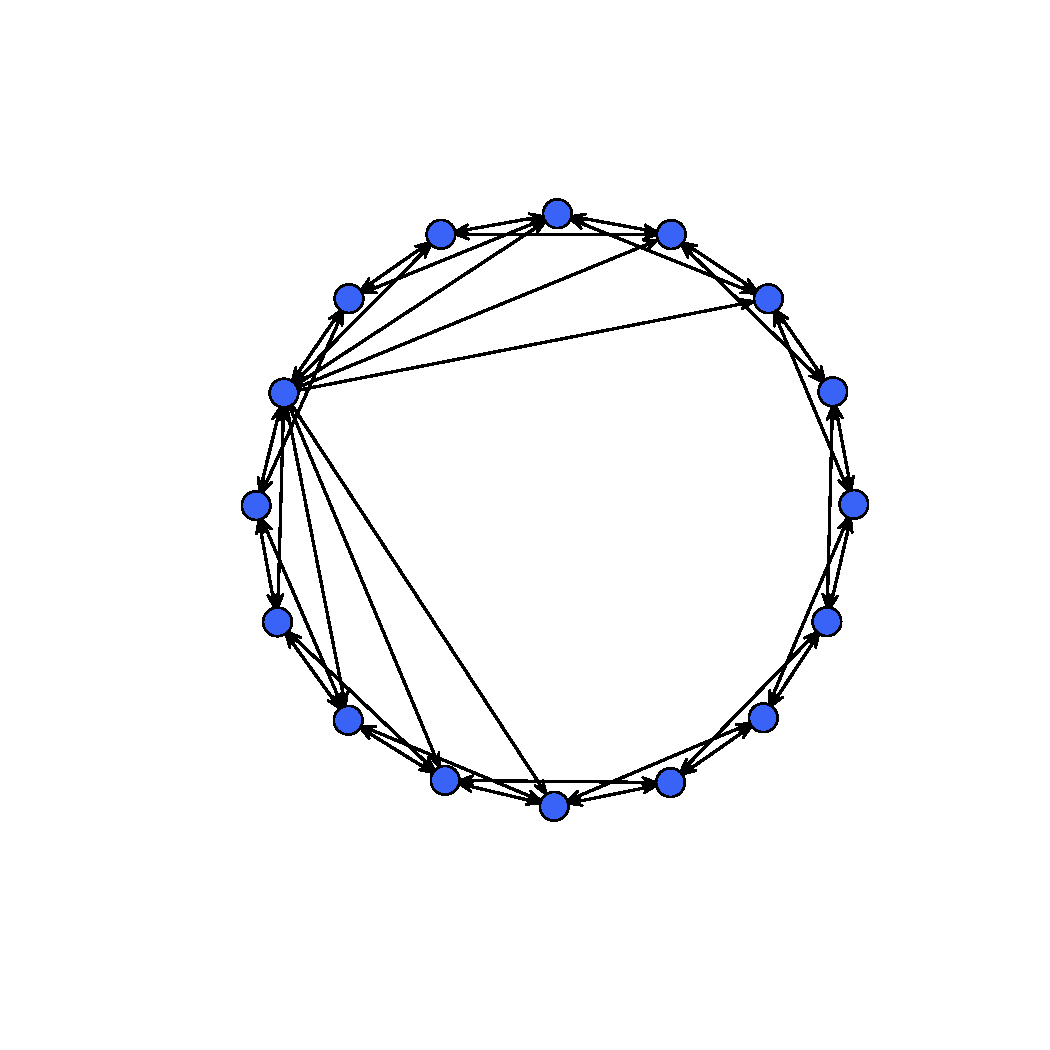
\includegraphics[width=.6\textwidth]{circle_w_invader.pdf}
\end{center}
\end{frame}

\begin{frame}
Optimizing $s_j$ affects everyone. 
%\begin{center}
\begin{columns}[c]
\column{.3\textwidth}
\column{.75\textwidth}
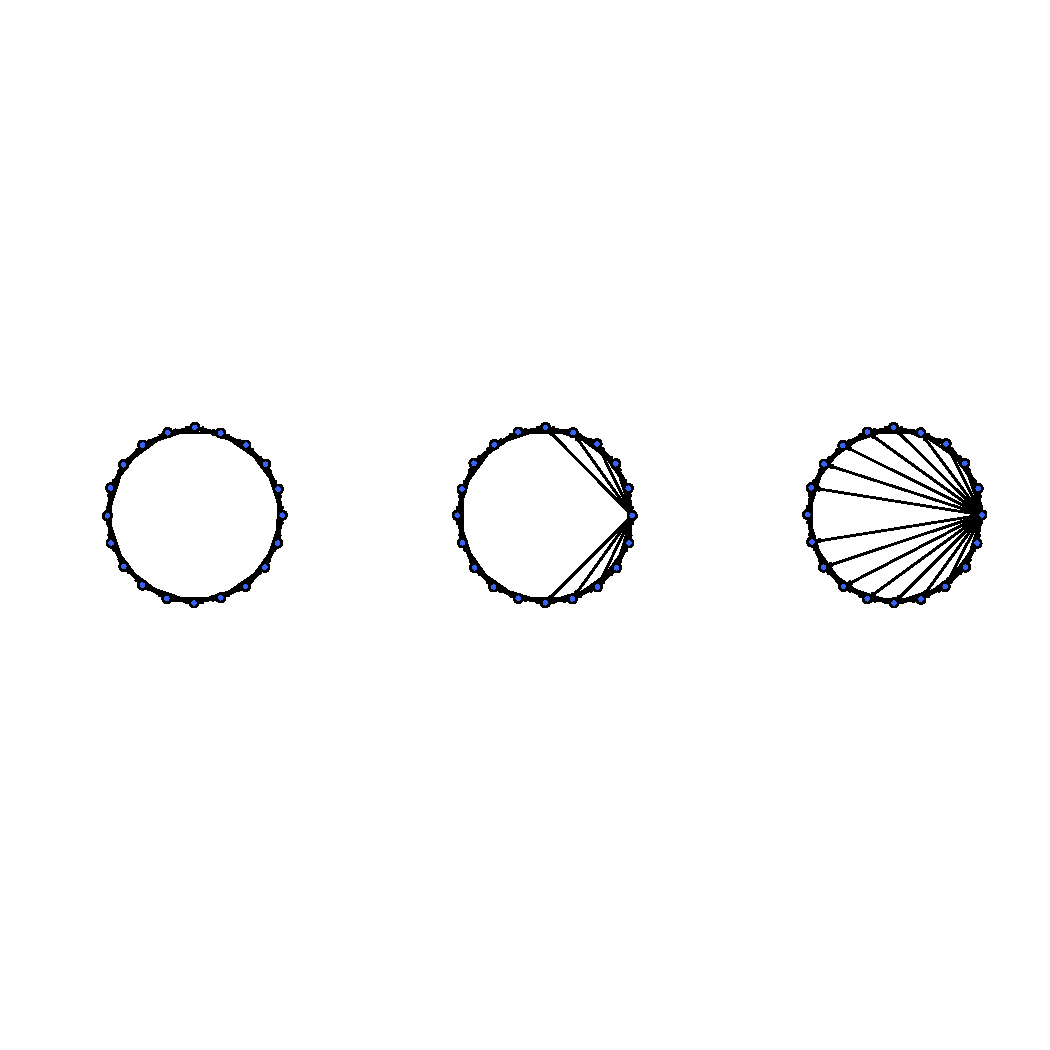
\includegraphics[width=\textwidth]{three_networks.pdf}
\end{columns}
%\end{center}
    \ra{1.3}
    \begin{tabular}{@{}clllllllllll@{}}
    $s_\text{invader}$  & & $0.2018$ & & & & $0.1993$ & & & & $0.1984$ 
    \\ $\langle s_j\rangle_{\text{native }j}$ & & $0.2018$ & & & & $0.2025$ & & & & $0.2029$
   \\ \small{$\lim_{t\to\infty} E[||y(t)||]$} & & $4.10$ & & & & $3.99$ & & & & $3.89$
    \\ \small{$\lim_{t\to\infty} E[||\delta(t)||]_{i=10}$} & & $5.98$ & & & & $5.48$ & & & & $5.09$
   \end{tabular}
\end{frame}


\begin{frame}
\begin{center}
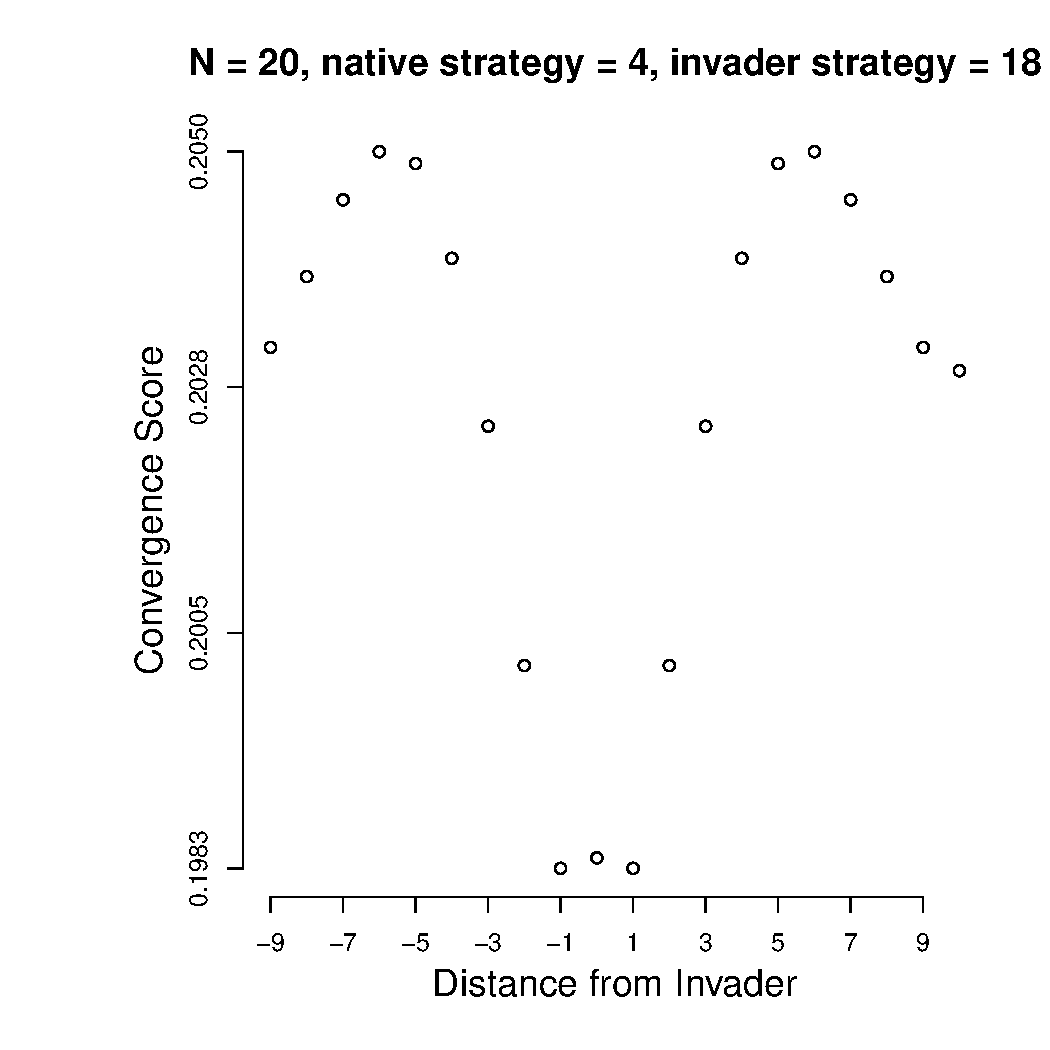
\includegraphics[width=.75\textwidth]{convergence_scores_one_network.pdf}
\end{center}
\end{frame}

\begin{frame}
\begin{center}$\small{\frac{\langle s_j\rangle _{\text{native }j}-s_\text{invader}}{\langle s_j\rangle _{\text{native }j}}}$ \end{center}
\begin{center}
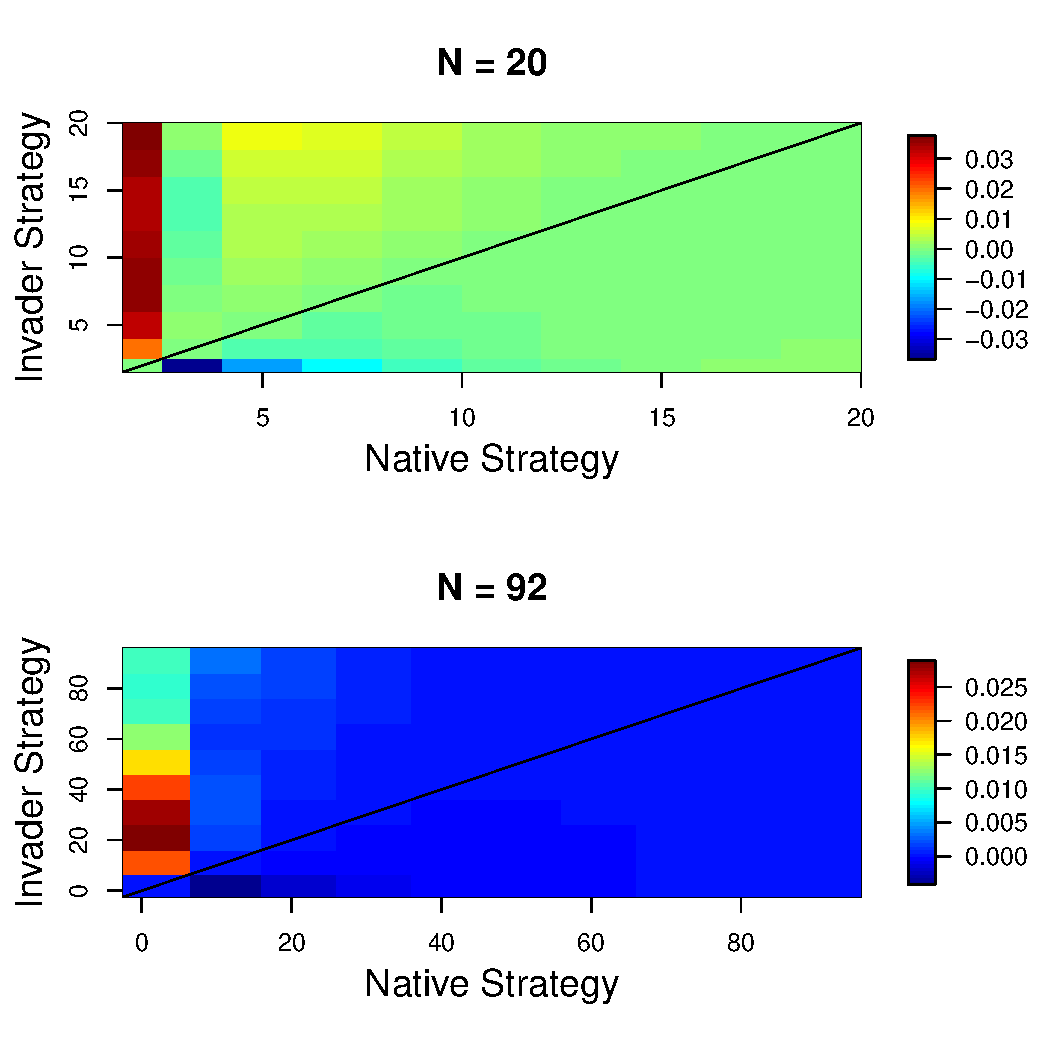
\includegraphics[width=.75\textwidth]{invader_advantage.pdf}
\end{center}
\end{frame}

\begin{frame}
\begin{center}
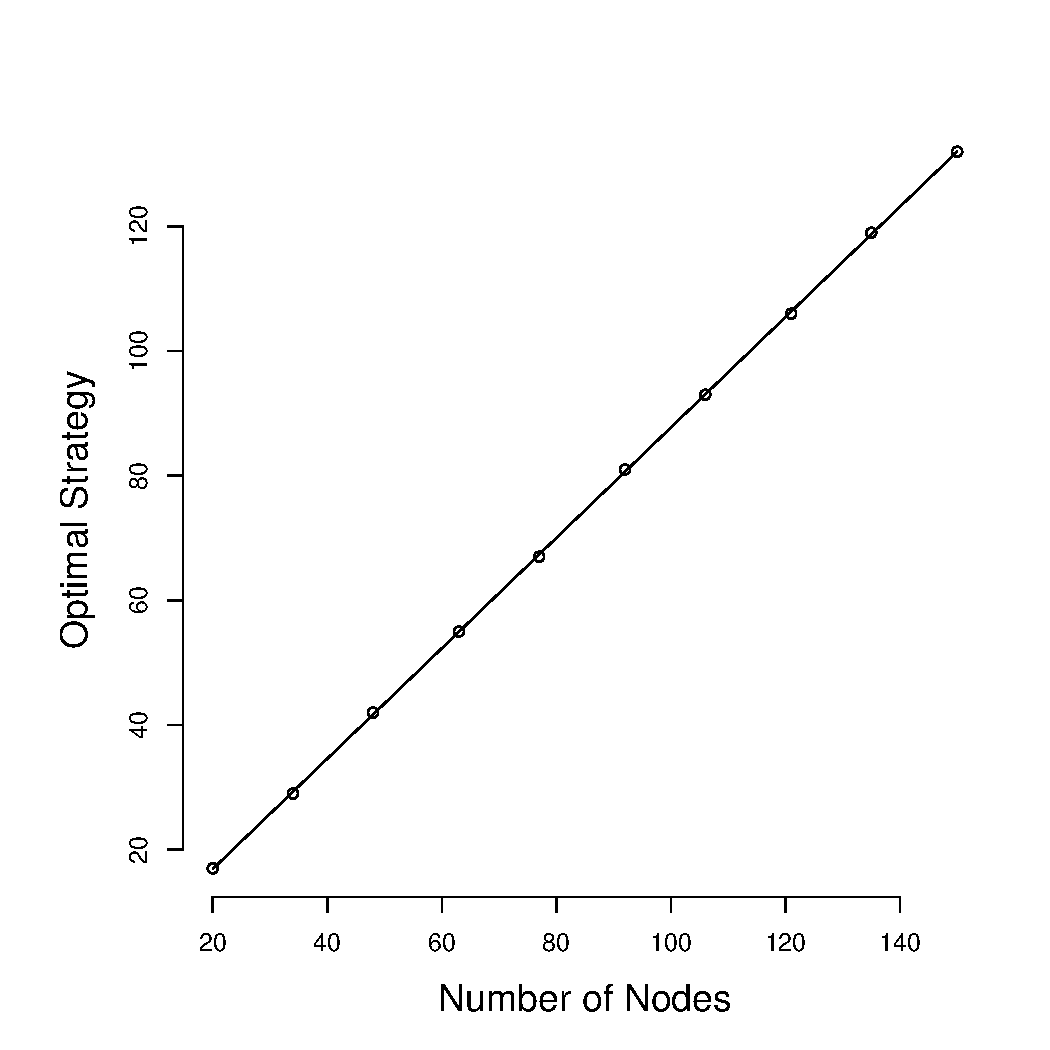
\includegraphics[width=.75\textwidth]{ESS_strategy.pdf}
\end{center}
\end{frame}

\begin{frame}
 \frametitle{Future Directions}
 \begin{itemize}
 \item allow for more variation among strategies across nodes and allow the strategies to evolve
 \item presence of multiple signals with different values 
 \item incorporate a principled measure of cognitive costs / informational burden of paying attention to more neighbors
 \item extend to other systems
 \item real network data
 \end{itemize}
 \end{frame}

\begin{frame}
\frametitle{Measure of Informational Burden}
\begin{align*}
&w_{ij}= \text{ weight of edge from } i\to j \ , \ \sum_jw_{ij}=1
\\& \Longrightarrow \text{ the vector $p$  such that } pW=p \text{ is the stationary distribution} 
 \\\\&\beta(W):= \text{ the entropy of the distribution }p \ , \ -\sum_ip_i\log(p_i)
\end{align*}

\end{frame}



\begin{frame}
\begin{center}
\includegraphics[width=.75\textwidth]{../../Documents/research/coarsegraining/compare_network_models.pdf}
\end{center}
\end{frame}


\begin{frame}
\frametitle{Future Directions}
\begin{itemize}
\item real network data
\item how to minimize informational burden while maintaining network structure
\item how informational constraints affects network inference
\end{itemize}
\end{frame}


\begin{frame}
\frametitle{Acknowledgements}
Simon Levin
\\Naomi Leonard
\\George Young
\end{frame}

\begin{frame}
\frametitle{$H_2$ norm}
Consider a dynamical system $\dot{v}(t)=Av+Bw$ and $z=Cv$.  Let $\Sigma$ be the solution to the Lyapunov equation $$A^T\Sigma+\Sigma A+BB^T=0.$$  Then the 
$H_2$ norm\footnote{Robustness of Noisy Consensus Dynamics with Directed Communication, Proceedings of the American Control Conference, George Forrest Young, Luca Scardovi, and Naomi Ehrich Leonard, 2010. } of the system is 
$$\sqrt{\tr(C\Sigma C^T)}.$$ 
For $y$, this means that $\Sigma$ solves $$-\overline{L}^T\Sigma-\Sigma\overline{L}+I=0 \text{ and } H_2=\sqrt{\tr(\Sigma)}.$$
It can be shown\footnotemark[\value{footnote}] that $H(L)=\lim_{t\to\infty}E[||y(t)||]=H_2(L).$

\end{frame}



\end{document}